\documentclass[11pt]{beamer}
\usepackage[utf8]{inputenc}
\usepackage[T1]{fontenc}
\usepackage{lmodern}
\usepackage[]{babel}
\usetheme{Madrid}
\usepackage{graphicx}
\begin{document}
	%\author{}
	\title{Heart Attack Analysis and Prediction Dataset}
	%\subtitle{}
	%\logo{}
	%\institute{}
	%\date{}
	%\subject{}
	%\setbeamercovered{transparent}
	%\setbeamertemplate{navigation symbols}{}
	\begin{frame}[plain]
		\maketitle
	\end{frame}
	
	\begin{frame}
		\frametitle{Correlation}
		% TODO: \usepackage{graphicx} required
		\begin{figure}
			\centering
			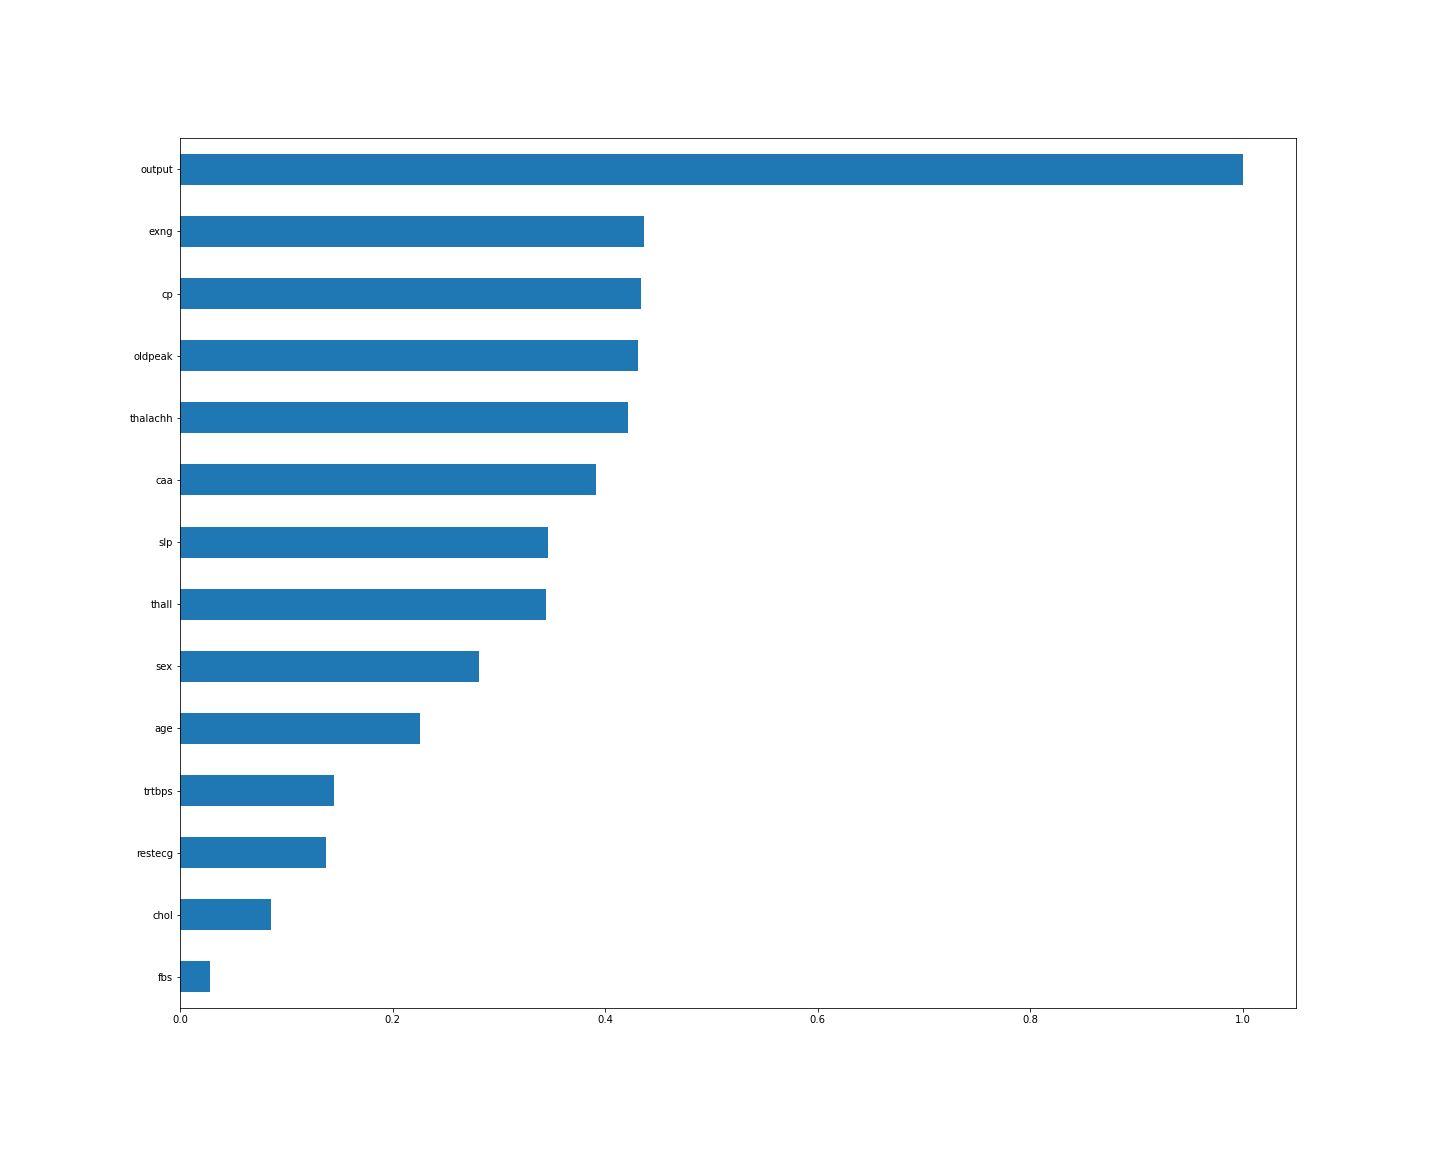
\includegraphics[width=0.7\linewidth]{C:/Users/KINGSLEY/OneDrive/Documents/GitHub/Heart-disease-ML-model/correlation}
			\caption{}
			\label{fig:correlation}
		\end{figure}
		\end{frame}
	\begin{frame}
		\begin{figure}
			\centering
			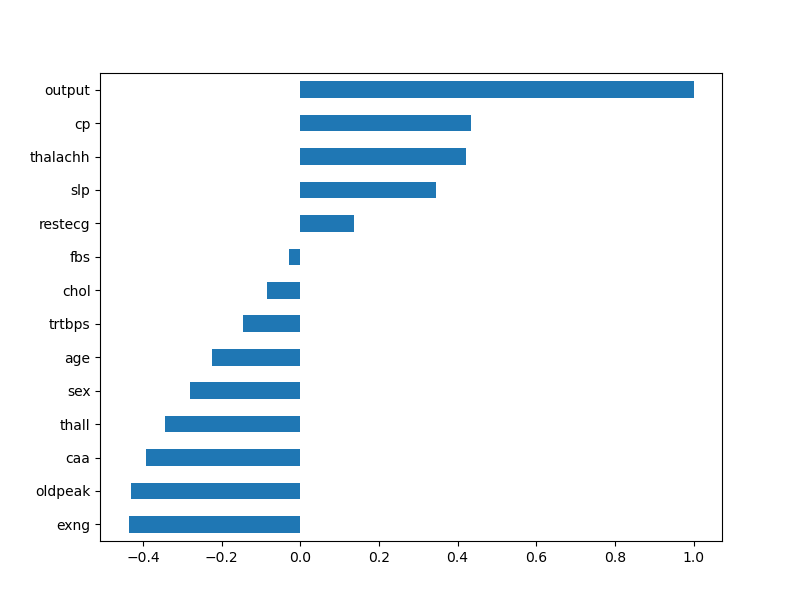
\includegraphics[width=0.7\linewidth]{C:/Users/KINGSLEY/OneDrive/Documents/GitHub/Heart-disease-ML-model/data/Figure_2}
			\caption{The Relation between the Features and the Target}
			\label{fig:figure2}
		\end{figure}
		
	\end{frame}
		
		\begin{frame}
			\begin{figure}
				\centering
				\includegraphics[width=0.7\linewidth]{C:/Users/KINGSLEY/OneDrive/Documents/GitHub/Heart-disease-ML-model/corrrr}
				\caption{Correlation Matrix of the Data}
				\label{fig:corrrr}
			\end{figure}
			
		\end{frame}
\begin{frame}
	\begin{figure}
		\centering
		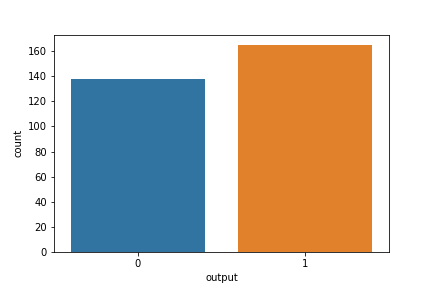
\includegraphics[width=0.7\linewidth]{C:/Users/KINGSLEY/OneDrive/Documents/GitHub/Heart-disease-ML-model/output}
		\caption{ Difference between the class of the Target}
		\label{fig:output}
	\end{figure}
	
\end{frame}

\begin{frame}
	\begin{figure}
		\centering
		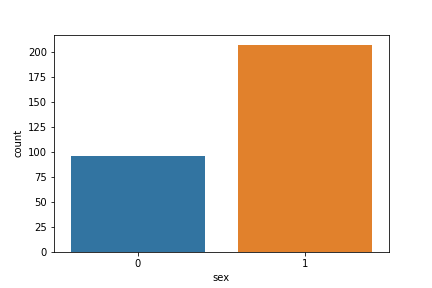
\includegraphics[width=0.7\linewidth]{C:/Users/KINGSLEY/OneDrive/Documents/GitHub/Heart-disease-ML-model/sex-output2}
		\caption{Difference between the Sex column of the data}
		\label{fig:sex-output2}
	\end{figure}
	
\end{frame}


\begin{frame}
	\begin{figure}
		\centering
		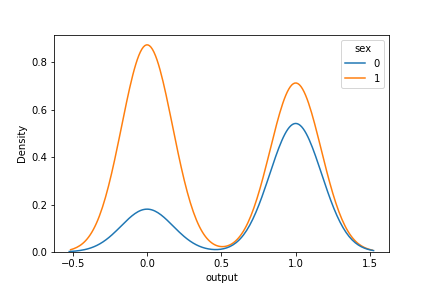
\includegraphics[width=0.7\linewidth]{C:/Users/KINGSLEY/OneDrive/Documents/GitHub/Heart-disease-ML-model/sex-output}
		\caption{}
		\label{fig:sex-output}
	\end{figure}
	
\end{frame}


\begin{frame}
	\begin{figure}
		\centering
		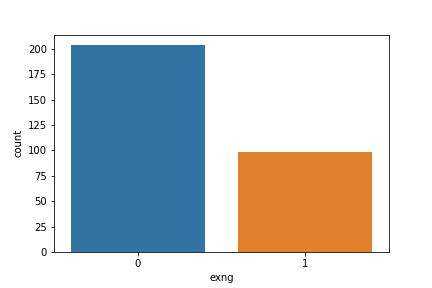
\includegraphics[width=0.7\linewidth]{C:/Users/KINGSLEY/OneDrive/Documents/GitHub/Heart-disease-ML-model/exng}
		\caption{exercise induced angina (1 = yes; 0 = no)}
		\label{fig:exng}
	\end{figure}
	
\end{frame}

\begin{frame}
	\begin{figure}
		\centering
		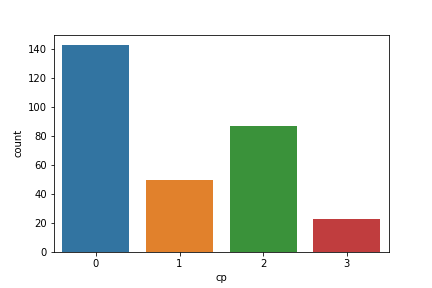
\includegraphics[width=0.7\linewidth]{C:/Users/KINGSLEY/OneDrive/Documents/GitHub/Heart-disease-ML-model/cp}
		\caption{Chest Pain Type}
		\label{fig:cp}
	\end{figure}
	
\end{frame}

\begin{frame}{Model Classification}
\begin{figure}
	\centering
	\includegraphics[width=0.7\linewidth]{C:/Users/KINGSLEY/OneDrive/Documents/GitHub/Heart-disease-ML-model/cor2}
	\caption{Confusion Matrix without Data Argumentation }
	\label{fig:cor2}
\end{figure}

\end{frame}

\begin{frame}
	\begin{figure}
		\centering
		\includegraphics[width=0.7\linewidth]{C:/Users/KINGSLEY/OneDrive/Documents/GitHub/Heart-disease-ML-model/comfffff}
		\caption{Improved Classifying after Data Argumentation }
		\label{fig:comfffff}
	\end{figure}
	
\end{frame}
\end{document}